% IEEE standard conference template; to be used with:
%   spconf.sty  - LaTeX style file, and
%   IEEEbib.bst - IEEE bibliography style file.
% --------------------------------------------------------------------------

\documentclass[letterpaper]{article}

\usepackage{spconf,amsmath,amssymb,graphicx,amsthm,newlfont,program,caption,subcaption}


% Example definitions.
% --------------------
% nice symbols for real and complex numbers
%\newcommand{\R}[0]{\mathbb{R}}
%\newcommand{\C}[0]{\mathbb{C}}


% bold paragraph titles
\newcommand{\mypar}[1]{{\bf #1.}}


\theoremstyle{definition}
\newtheorem{observation}{Observation}

\newtheorem{algorithm}{Algorithm}


% Title.
% ------
\title{A Descriptive Title, not too general, not too long}
%
% Single address.
% ---------------
\name{Markus P\"uschel\thanks{The author thanks Jelena Kovacevic. This paper
is a modified version of the template she used in her class.}} 
\address{Department of Computer Science\\ ETH Z\"urich\\Z\"urich, Switzerland}

% For example:
% ------------
%\address{School\\
%		 Department\\
%		 Address}
%
% Two addresses (uncomment and modify for two-address case).
% ----------------------------------------------------------
%\twoauthors
%  {A. Author-one, B. Author-two\sthanks{Thanks to XYZ agency for funding.}}
%		 {School A-B\\
%		 Department A-B\\
%		 Address A-B}
%  {C. Author-three, D. Author-four\sthanks{The fourth author performed the work
%		 while at ...}}
%		 {School C-D\\
%		 Department C-D\\
%		 Address C-D}
%

\begin{document}
%\ninept
%
\maketitle
%

The hard page limit is 6 pages in this style. Do not reduce font size
or use other tricks to squeeze. This pdf is formatted in the American letter format, so the spacing may look a bit strange when printed out.

\begin{abstract}
Describe in concise words what you do, why you do it (not necessarily
in this order), and the main result.  The abstract has to be
self-contained and readable for a person in the general area. You
should write the abstract last.
\end{abstract}

\section{Introduction}\label{sec:intro}

Do not start the introduction with the abstract or a slightly modified
version. It follows a possible structure of the introduction. 
Note that the structure can be modified, but the
content should be the same. Introduction and abstract should fill at most the first page, better less.

\mypar{Motivation} The first task is to motivate what you do.  You can
start general and zoom in one the specific problem you consider.  In
the process you should have explained to the reader: what you are doing,
why you are doing, why it is important (order is usually reversed).

For example, if my result is the fastest sorting implementation ever, one
could roughly go as follows. First explain why sorting is important
(used everywhere with a few examples) and why performance matters (large datasets,
realtime). Then explain that fast implementations are very hard and
expensive to get (memory hierarchy, vector, parallel). 

Now you state what you do in this paper. In our example: 
presenting a sorting implementation that is
faster for some sizes as all the other ones.

\mypar{Related work} Next, you have to give a brief overview of
related work. For a report like this, anywhere between 2 and 8
references. Briefly explain what they do. In the end contrast to what
you do to make now precisely clear what your contribution is.

\section{Background: Whatever the Background is}\label{sec:background}

Give a short, self-contained summary of necessary
background information. For example, assume you present an
implementation of sorting algorithms. You could organize into sorting
definition, algorithms considered, and asymptotic runtime statements. The goal of the
background section is to make the paper self-contained for an audience
as large as possible. As in every section
you start with a very brief overview of the section. Here it could be as follows: In this section 
we formally define the sorting problem we consider and introduce the algorithms we use
including a cost analysis.

\mypar{Sorting}
Precisely define sorting problem you consider.

\mypar{Sorting algorithms}
Explain the algorithm you use including their costs.

As an aside, don't talk about "the complexity of the algorithm.'' It's incorrect,
problems have a complexity, not algorithms.


\section{Your Proposed Method}\label{sec:yourmethod}

The purpose of this section is to review a convex hull sequential algorithm for a sorted input set and common tangent line algorithm. We also present parallel algorithms for computing a convex hull for such input.

\subsection{Sequential algorithm}
% TODO(matalek): do we want to include that?

\subsection{Common tangent line algorithm}

\subsection{Parallel algorithms}

Algorithms presented here enable computing the upper hull of the input set. 
Computing lower hull can be done in a similar way and for simplicity its description is omitted in this report. 
Therefore, in this section, whenever we write ''convex hull'' we are referring to the upper hull.
However, our implementation computes the entire convex hull (upper and lower).  

\subsubsection{General scheme}
\label{sec:parallel-general}

Let $k$ denote the number of processors used and $n$ - number of points in the input set.
For simplicity in all algorithms we will assume that $k$ is the power of 2. 
Let $P = \{p_0, p_1, ..., p_{n-1} \}$ be the set of sorted (by $x$ coordinate) input points.
Finally, let $CH(S)$ denote the convex hull of $S$ set and $R=CH(P)$.
All presented here algorithms share a common approach.

Firstly, we divide the input set into $k$ equal sets ($\pm 1$ elements) based on the $x$ coordinate:
$$P_0 = \{p_0, p_1, ..., p_{\lceil{\frac{n}{k}}\rceil - 1}\}$$
$$P_1 = \{p_{\lceil{\frac{n}{k}}\rceil}, p_{\lceil{\frac{n}{k}}\rceil + 1}, ..., p_{\lceil{2 * \frac{n}{k}}\rceil - 1}\}$$
$$...$$
$$P_{k-1} = \{p_{(k-1)\lceil{\frac{n}{k}}\rceil}, p_{(k-1)\lceil{\frac{n}{k}}\rceil + 1}, ..., p_{n- 1} \}$$


Then, we execute sequential version of the convex hull algorithm (Andrew's monotone chain) for each of these sets in parallel, using $k$ threads.
As a result we have the convex hull for each of the sets:
$$C_i = CH(P_i) \textrm{\;\;\; for \;} i \in \{0, 1, ..., k - 1\}$$

For the next step we need the following simple observation:
\begin{observation}
If $p \in P_i$ for some $i \in \{0, 1, ..., k - 1\}$, but $p \notin C_i$, then $p \notin R$.
\end{observation}

The immediate conclusion follows:
\begin{observation}
$$R = CH(C_0 \cup C_1 \cup ... \cup C_{k - 1})$$
\end{observation}

This observation enables us to perform the last step of the algorithm.
It consists of merging partial convex hulls $C_0, C_1, ..., C_{k - 1}$ into one convex hull $R$.
This is the step, where our algorithms differ.
Each of the algorithm presents different ways of merging partial convex hulls.
All of them are, however, based on the common tangent line algorithm.

\subsubsection{Naive Parallel algorithm}

So called Naive Parallel algorithm is based on merging two convex hulls into one convex hull.
It uses common tangent line algorithm, but the overall concept was developed by us.
% TODO(matalek): phrase above maybe somehow better

Let $A$ and $B$ be two convex hulls so that for every $p \in A, q \in B$ we have $p.x < q.x$, where $r.x$ denotes the $x$ coordinate of the point $r$.
Further, let $p_0, p_1, ..., p_{n-1}$ and $q_0, q_1, ... q_{m-1}$ be the points of $A$ and $B$ respectively (sorted by $x$ coordinate).
Let $p_i \in A$ and $q_j \in B$ be such points that $\overline{p_iq_j}$ is a common tangent line for $A$ and $B$.
Then we know that points $p_{i+1}, p_{i + 2}, ..., p_{n - 1}$ and $q_{j + 1}, q_{j + 2}, ..., q_{m - 1}$ are not going to be in the resulting convex hull.
Therefore, we have:
$$CH(A \cup B) = \{ p_0, p_1, ..., p_{i - 1}, p_i, q_j, q_{j + 1}, ..., q_{m - 1} \}$$
For performing this merge we can use array-like data structure.
The time complexity of this is equal to $O(n + m)$.
% TODO(matalek): is it true? check with common tangent line complexity

Using this merge algorithm we can compute the convex hull of the entire set in the form of the tree.
Our algorithm consists of $\log k$ steps.
We start with $C_0, C_1, ..., C_{k-1}$ convex hulls.
In each step we are merging convex hull which were pairs of resulting convex hulls from the previous step. 
If $I_0, I_1, ..., I_{2l - 1}$ is the input for the step, then we compute the output: $O_0, O_1, ..., O_{l - 1}$ using $l$ processors. 
$i$-th processor computes $O_i = CH(I_{2i} \cup I_{2i+1})$ using merge algorithm presented above.
Example scheme for 4 processors is presented on figure \ref{fig:naive-parallel-scheme}.
Pseudocode for this algorithm is presented as algorithm \ref{alg:naive-parallel}.

% TODO(matalek): think if we should put it without page break.
\begin{algorithm}
\label{alg:naive-parallel}
\begin{program}
\mbox{NaiveParallel algorithm:}
\BEGIN \\ %
  level := k / 2;
  partial\_results := array(2 * k);
  \FOR i := 0 \TO level \STEP 1 \textrm{\bf{\;in parallel}} \DO
    partial\_results[k + i] := 
    \;\;\;\; sequential\_algorithm(input, i)
  \OD
  \WHILE level > 0 \DO
    \FOR i := 0 \TO level \STEP 1 \textrm{\bf{\;in parallel}} \DO
      pos = level + i;
      partial\_results[pos] := merge(
      \;\;\;\; partial\_results[2*pos],
      \;\;\;\; partial\_results[2 * pos + 1])
    \OD
    level /= 2;
  \OD
  print(partial\_results(1));

\END
\end{program}
\end{algorithm}

\begin{figure}\centering
  \includegraphics[scale=0.5]{img/naive-parallel}
  \caption{Scheme of merging convex hulls for $k=4$}
  \label{fig:naive-parallel-scheme}
\end{figure}

The time complexity of this algorithm depends on the size of intermediates convex hulls.
In the worst case scenario size of the convex hull will be linear to the size of the input.
Then, time complexity of the algorithm can be estimated as:
$$O(\frac{n}{k}) + O(2\frac{n}{k}) + O(4\frac{n}{k}) + ... + O(k\frac{n}{k}) = O(n)$$
We can see that asymptotically this algorithm in the worst case scenario does not provide any speedup when using more threads.
However, as shown and explained in next sections, this algorithm proved to be quite efficient.

\subsubsection{Simple Parallel algorithm}
\label{sec:simple-parallel}

This algorithm was originally presented in \cite{SimpleParallel}.
It is based on computing what part of $C_i$ is also a part of $R$.
The computations are based on the following observation:
\begin{observation}
Let $C_i = \{q_0, q_1, ..., q_{l-1} \},$ where  $q_{j_1}.x < q_{j_2}.x$ for $0 \leq j_1 < j_2 < l$. 
We have, that for every $0 \leq j_1 < j_2 < j_3 < l$, if $q_{j_1}, q_{j_3} \in R$, then $q_{j_2} \in R$.
% TODO(matalek): do we need proof for it?
\end{observation}
We will call a point $p$ {\it\bf taken} if and only if $p \in C_i \land p \in R$ for some $i$. 
The above observation means that taken points from one convex hull form an interval (with regards to their indices).

Computing these intervals can be done by computing common tangent line for each pair $C_i$ and $C_j$.
For these pairs we know how  to compute intervals of taken points (see previous section). 
For given $i$ we can then compute intersection of the intervals computed for $C_i$ and $C_j$ for every $i \neq j$.
Let $[j_1, j_2]$ be the interval of indices corresponding to the calculated intersection.
If $j_1 < j_2$ then this interval corresponds also to the interval of taken points.
However, when $j_1 = j_2$ there might be two possible cases.
They are illustrated on the figure \ref{fig:simple-parallel}.
In the first case we have that the appropriate point is taken, in the second one - it is not.
The difference between these cases is the angle that common tangents line are forming.
In the first case, when going from left to right the angle between two steepest common lines is less than $\pi$, in the second case it is greater or equal $\pi$.
This means, that in the algorithm we need to keep track also of the steepest common tangent lines and use this information for this special case.
Solution for this special case was not presented in $\cite{SimpleParallel}$ and is originally developed by us.
% TODO(matalek): is above correct?

\begin{figure}
\centering
\begin{subfigure}{.3\textwidth}
	\centering
	\includegraphics[width=\linewidth]{img/simple-parallel-taking}
	\caption{Point with index $j_1$ is taken}
\end{subfigure}
\begin{subfigure}{.3\textwidth}
	\centering
	\includegraphics[width=\linewidth]{img/simple-parallel-not-taking}
	\caption{Point with index $j_1$ is not taken}
\end{subfigure}
\caption{Different possibilities for $j_1 = j_2$}
\label{fig:simple-parallel}
\end{figure}

These computations are done in parallel.
Processor $i$ computes all intervals for $C_i$ and $C_j$, where $j = 0, 1, ..., i -1, i+ 1, ..., k - 1$ and then computes their intersection.

The last steps consist of moving all taken points to one resulting array.
Firstly, we compute how many points from each convex hull $C_i$ are taken.
Let the result of this computation be: $l_1, l_2, ..., l_{k-1}$.
We can then compute starting positions in the resulting array for each taken points set from one convex hull.
Taken points from $C_i$ should be put at indices from $l_1 + l_2 + ... + l_{i-1}$ to $l_1 + l_2 + ... + l_{i-1} + l_i - 1$.
Calculating these indices can be done using parallel prefix computation.
We later copy taken points to the resulting array in parallel - each processor copies points from its own convex hull.


The time complexity for this algorithm, as shown in \cite{SimpleParallel}, is equal $O(\frac{n}{k} + k(\log \frac{n}{k})^2)$ and is optimal for $k \leq \frac{\sqrt{n}}{\log n}$.

\subsubsection{Hull Tree algorithm}

This algorithm was originally presented in \cite{HullTree}.
It is based on a special tree-like structure for keeping points of the convex hull.
Let $n$ denote the number of points in the convex hull.
This data structure allows:
\begin{itemize}
\item creating a new hull tree from a convex hull represented as an array, in $O(n)$ time complexity,
\item accessing leftmost and rightmost point, in $O(\log n)$ time complexity,
\item accessing neighboring (with regards to the position on the convex hull) points, in $O(1)$ time complexity,
\item creating a hull tree consisting of subset of points from the original hull tree that have $x$ coordinate lower than given one, in $O(\log n)$ time complexity,
\item merging two hull trees, where one of them consists of points that have $x$ coordinate lower than all the points from the second one, in $O(\log n)$ time complexity, where $n$ and $m$ are the number of points in the hull trees to be merged.
\end{itemize}
The details of implementation of this data structure are presented in the original paper.
% TODO(matalek): is paper a good word?

This algorithm uses divide and conquer approach. 
Let $d = \lceil\frac{n}{k}\rceil$ and $S$ be the current set of input points.
If the size of $S$ is lower or equal than $d$, we execute a sequential version of the algorithm and construct a hull tree based on its result.
Otherwise, we split $S$ into $\sqrt{k}$
equal subsets based on $x$ coordinate: $S_0, S_1, ..., S_{\sqrt{k} - 1}$
\footnote{More precisely, we split into $O(\sqrt k)$ sets. In our implementation for $k \geq 4$ we split into $2^w$ sets, where $w$ is the highest number such that $2^{2w} \leq k$ (for $k = 2$ we split into 2 sets).}.
We then compute recursively convex hull for each subset, which results in having hull trees $HT_i$ corresponding to convex hulls $C_i$ of these subsets.
For each recursive call we assign $\sqrt{k}$ processors to compute this convex hull.

In order to merge $HT_0, HT_1, ..., HT_{\sqrt{k} - 1}$ we perform computations similar to these described in the section \ref{sec:simple-parallel}.
Using $\sqrt{k}^2 = k$ processors we compute for each pair $HT_i$ $HT_j$ ($i \neq j$) common tangent line (for each pair we assign one processor).
It is possible to perform this step efficiently, because our data structure enables us to quickly access neighboring points, as well as middle points of given interval of points.
Later, we compute the intersection of resulting intervals which results in the intervals of taken points.
If $q_1$ and $q_2$ are the beginning and the end of one of these intervals, we split hull tree first by $q_1.x$ and discard left convex hull, later by $q_2.x$ and discard right resulting convex hull.
We are left then with hull tree representing only taken points.
We merge these hull trees in a tree-like way (similar to described in the section \ref{sec:parallel-general} and pairwise merge of hull trees.
These operations are performed in parallel by $\sqrt{k}$ processors and take $O(h + k)$ time.
Finally, using parallel prefix computation we copy points from the resulting hull tree into the resulting array.

The time complexity for this algorithm, as shown in \cite{HullTree}, for $k \leq \frac{n}{\log n}$ is equal $O(\frac{n}{k})$ and is optimal.

\iffalse
Now comes the ``beef'' of the report, where you explain what you
did. Again, organize it in paragraphs with titles. As in every section
you start with a very brief overview of the section.

In this section, structure is very important so one can follow the technical content.

Mention and cite any external resources that you used including libraries or other code.
\fi

\section{Experimental Results}\label{sec:exp}
%TODO (matalek) say why naive is good hull is bad
In order to evaluate the efficiency of our proposed algorithms, we tested them on sets of randomly generated points with different geometric shapes: square, disk and circle.

Regarding scalability we tested both weak and strong scaling, changing the input size and the number of operating threads.

Concerning correctness we compared our results with the ones obtained using th \textit{Convex Hull} implementation available in the library \textit{CGAL} \footnote{http://www.cgal.org/}.

\subsection{Experimental setup}

%TODO
The platform we tested our algorithms with mounts Intel$^{(R)}$ Xeon Phi processors. They are based on the Intel$^{(R)}$ Many Integrated Core (MIC) architecture.

\begin{table}[!ht]
\begin{tabular}{|c|c|}
\hline Number of cores			& 61\\
\hline Threads					& 244\\
\hline Model name				& Intel(R) Xeon Phi 7100\\
\hline CPU Frequency [MHz]		& 1238.094\\
\hline Cache size [KB]			& 512\\
\hline Peak Performance [GFlops]	& 1208\\
\hline Peak memory bandwidth [GB/s]		& 352\\
\hline
\end{tabular}
\caption{Xeon Phi cluster specifications}
\end{table}

Our implementations are written in \textit{C++11} and make use of \textit{OpenMP} ver 4.0 \footnote{http://www.openmp.org/} for shared-memory multithreading.
Our applications were compiled using \textit{icc} version 15.0.0 with the flag \textit{-O2} using also the -mmic flag to fit the architecture.

This is roughly how our experiments worked:
first of all we fixed a shape and a number of points to be generated. Then we randomly generated the chosen point set and executed each algorithm with each desired number of threads on that point set, collecting results in logfiles, measuring two time intervals: \textit{mid} (the time needed for the first part of the algorithms that is the separated computing of convex hulls) and \textit{end} (the time needed for merging results).

In order to have reliable experiments we repeated this process 100 times for each chosen combination of number of input points and shape.

This whole process was done for 10$^4$, 10$^5$, 10$^6$ and 10$^7$ points with integral coordinates and different $x$ coordinates generated in a range R of 10$^9$ and as shapes we used square, disk and circle in the following way:

\mypar{Square}: Randomly generated points with coordinates in the range [-R,R]

\mypar{Disk}: Randomly generated points with coordinates in the range [-R,R]. Points not included in the disk with radius R and center (0,0) were removed and regenerated.

\mypar{Circle}: Randomly generated angles $\theta_n$ and created the points ($\frac{R}{2}cos(\theta_n)$, $\frac{R}{2}sin(\theta_n)$).

These shapes were chosen because of the difference in the resulting hulls.
With square, in fact, resulting hulls are very small, while with the circle almost every input point is part of the final hull (some point will be excluded because of approximation of integers) and for disk resulting hulls have intermidiate size.

\subsection{Results}

Here we show how our algorithms perform under different configurations and with weak and strong scaling.
The results plotted are the arithmetic averages of the 100 different repetitions performed for each configuration (Input shape, input size, algorithm and number of processing threads).

Results obtained with disks as input are not shown because close to identical to the squares' ones.

The sequential version considered is the \textit{Andrew's Monotone Chain} algorithm that's used inside our parallel algorithms. \textit{Andrew's Monotone Chain} is also used as base case for speedup plots.

\subsubsection{General results and reliability}

Put BOXPLOTS HERE???

\subsubsection{Changing input size for fixed number of threads}

Here we analyze the results of our algorithms when changing input size from 10$^4$ to 10$^7$ points. We show performance with 8 processing threads to represent the trends of the algorithms, which is generally the same (with different speedups) for the tested number of threads.

\begin{figure}[!ht]\centering
  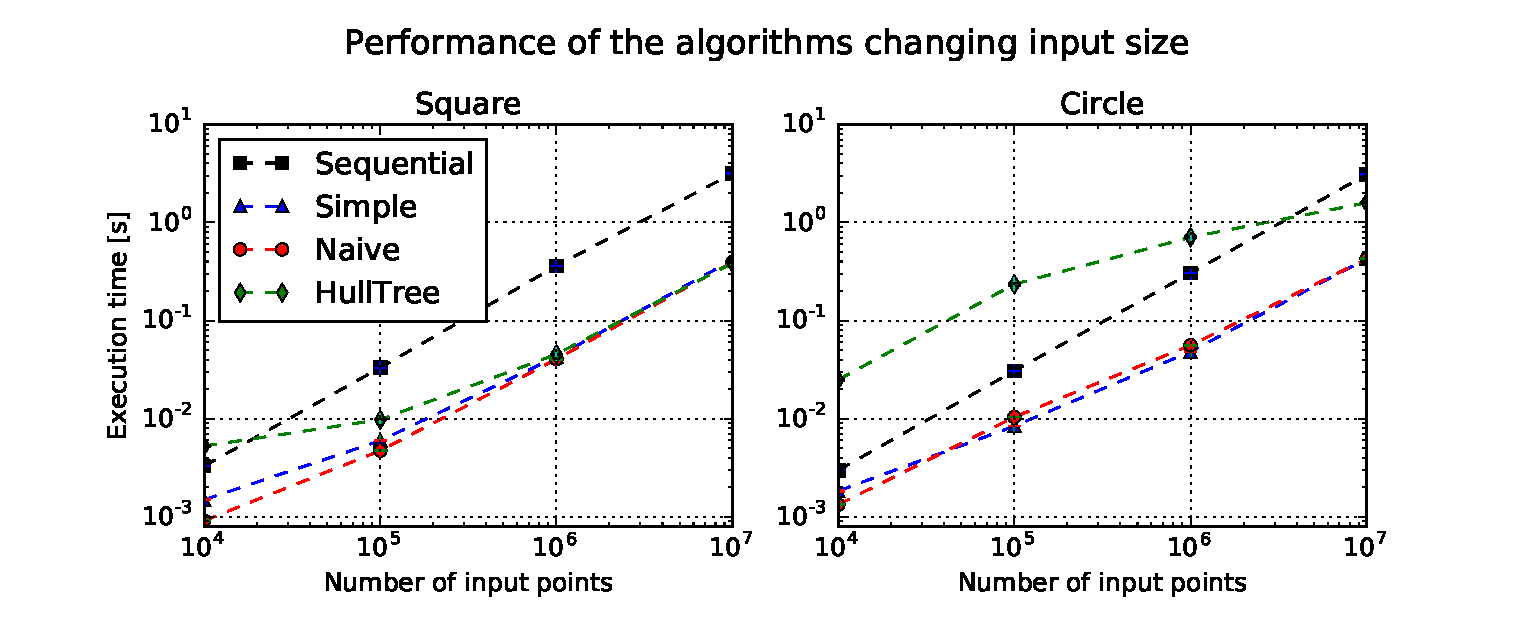
\includegraphics[scale=0.33]{./plots/time_points.eps}
  \caption{Comparison of the execution times three algorithms for 8 threads and the sequential version changing input size for square and circle\label{Input size time}}
\end{figure}

For the sequential versions the growth in execution time when increasing the number of input points is linear for all the selected shapes.
Concerning the parallel algorithms they have similar trends except for \textit{HullTree}, that performs significantly worse for small input sets [Plot \ref{Input size time}], expecially with the circle: \textit{HullTree}'s performance is even worse than the sequential one.
This is due to the creation of the data structure that for a high number of resulting points (recall that for circle almost every generated point is part of the final convex hull) needs a lot of time.

\begin{figure}[!ht]\centering
  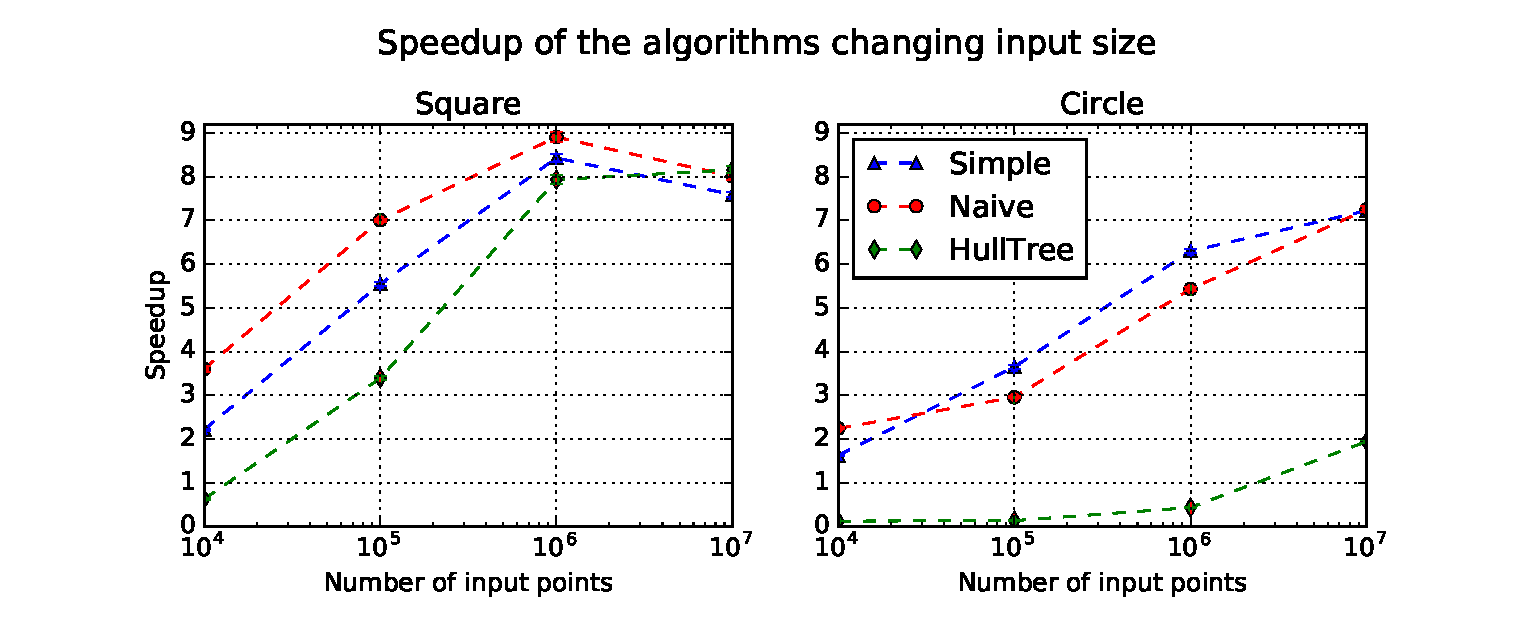
\includegraphics[scale=0.33]{./plots/speedup_points.eps}
  \caption{Speedup comparison of the three algorithms for 8 threads changing input size for square and circle\label{Input size speedup}}
\end{figure}

Looking at the speedup plots [Plot \ref{Input size speedup}] the general trend is a general growth in efficiency when increasing the size of the input set for the two shapes.

We notice a superlinear speedup around 10$^6$ points (around 9 for \textit{Naive} and 8.5 for \textit{Simple}) and 10$^7$ points (slightly above 8 for both \textit{Simple} and \textit{HullTree}.
We obtained superlinear speedup thanks to caching: splitting the input set into smaller subsets assigned to processors makes the subset fit better into cache, allowing faster accesses to the points.

\subsubsection{Change number of threads for fixed input}

Here we analyze the performance of our algorithms with the different number of processing threads under a fixed input size of 10$^6$ and 10$^7$ points.

\begin{figure}[!ht]\centering
  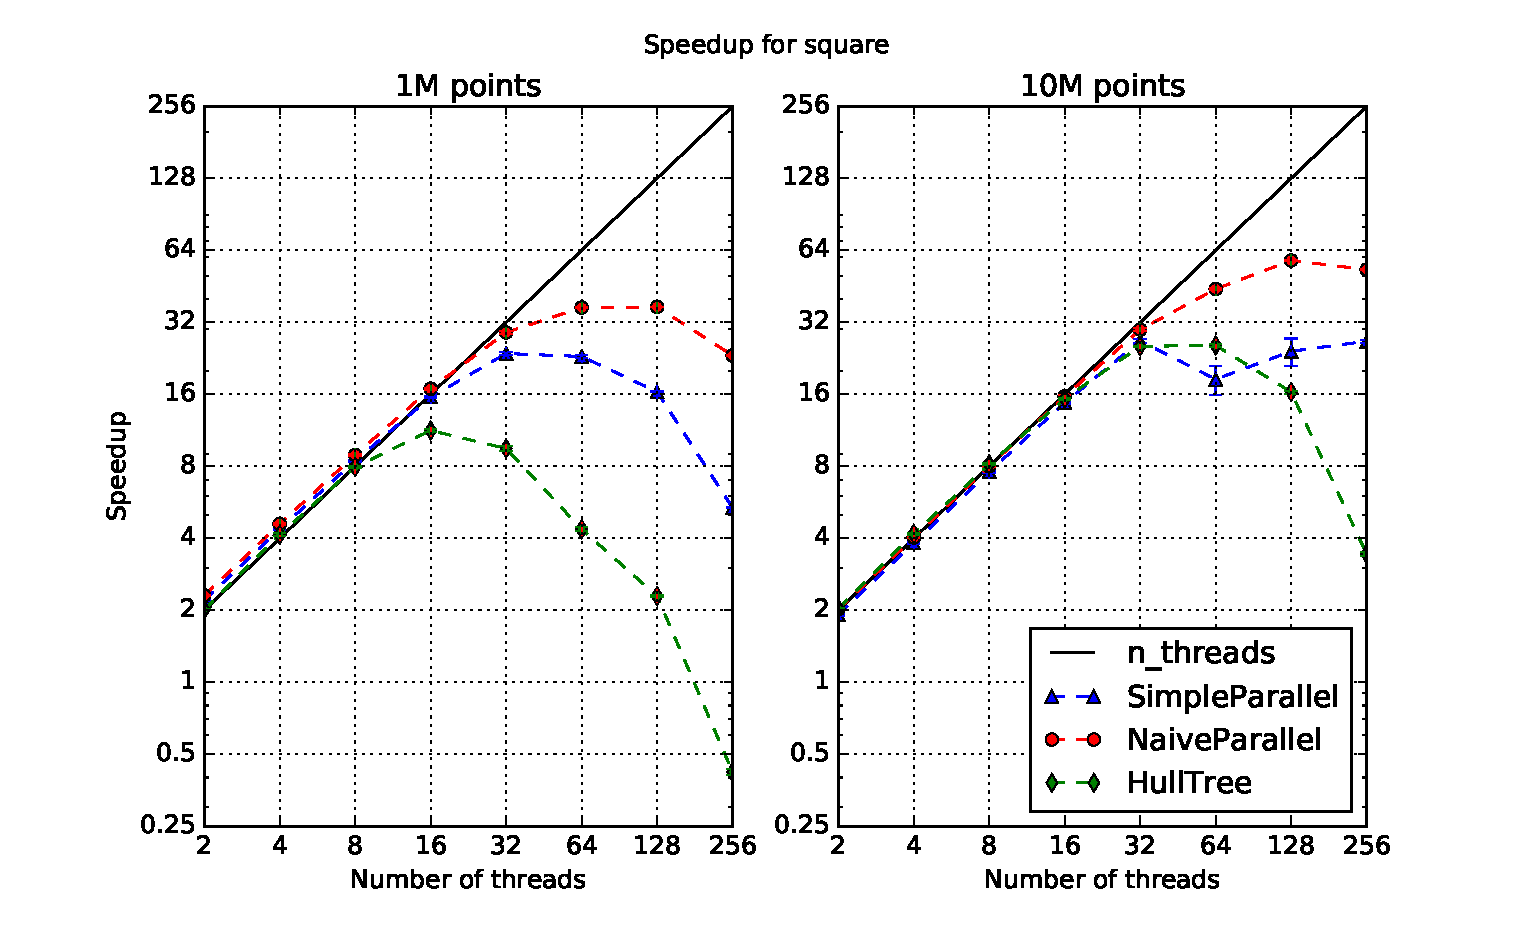
\includegraphics[scale=0.33]{./plots/speedup_xeon_square_fixed_points.eps}
  \caption{Speedup of the algorithms with the given number of threads with a square for 10$^6$ [Sequential execution time: 0.3s] and 10$^7$ [sequential execution time: 3s] points\label{Threads speedup square}}
\end{figure}

For square and disk we notice similar trends [Plot \ref{Threads speedup square}] speedup close to linear or even superlinear until around 16 threads for 10$^6$ points and 32 for 10$^7$ points then a general decrease in efficiency growth up to a point where our algorithms stop scaling and the speedup starts decreasing.

We can notice that that point is shifted to a higher number of threads when the input set is bigger. Clearly the lower the number of points the lesser the efficiency obtained by splitting the point set among threads.
After that point, the overhead added by parallelism overweights the benefits introduced by having more processing units.

This overhead is related both to the Operating System, that has to create, allocate and manage a high number of threads, and to the algorithms themselves:
in fact for a high number of threads, while the first part of the algorithms (separately compute convex hull on split point sets) becomes very fast, the merging itself takes more time and the two processes start becoming unbalanced.

\begin{figure}[!ht]\centering
  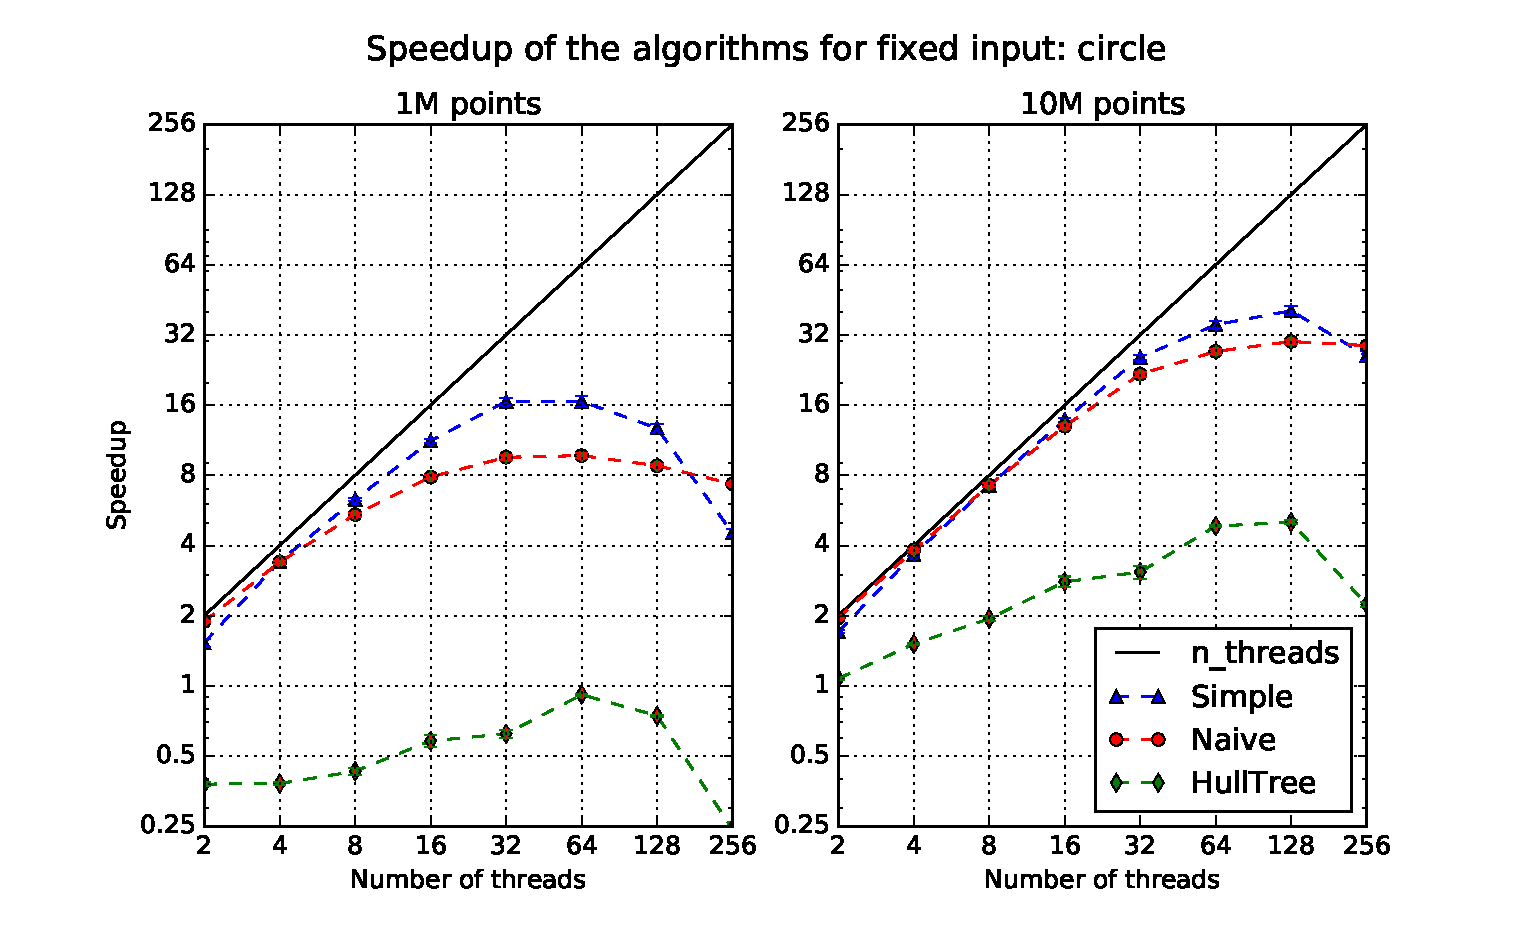
\includegraphics[scale=0.33]{./plots/speedup_xeon_circle_fixed_points.eps}
  \caption{Speedup of the algorithms with the given number of threads with a circle for 10$^6$ [sequential execution time: 0.3s] and 10$^7$ [sequential execution time: 3s] points\label{Threads speedup circle}}
\end{figure}

For circle [Plot \ref{Threads speedup circle}] the situation is again more complicated, since the HullTree algorithm has a very bad performance, but the trend is very simlar with a fast increase in efficiency followed by a close-to-steady state and a decrease in efficiency for a high number of threads.
Quantitatively the overall efficiency of the parallel algorithms is lower than the one obtained with the square and that's probably because the more memory accesses needed and the parallel overhead make the algorithms behave worse.

\subsubsection{Behavior with unoptimal number of threads}

For a number of threads that is not a power of 2, because of their implementations, Naive and HullTree algorithm behave like the closest lower power of two (i.e. with 35 threads they behave like they had 32).

\textit{Simple} algorithm, instead, is not correlated to powers of two and the performance for any number of threads is ?????????????????????????????.

\begin{figure}[!ht]\centering
  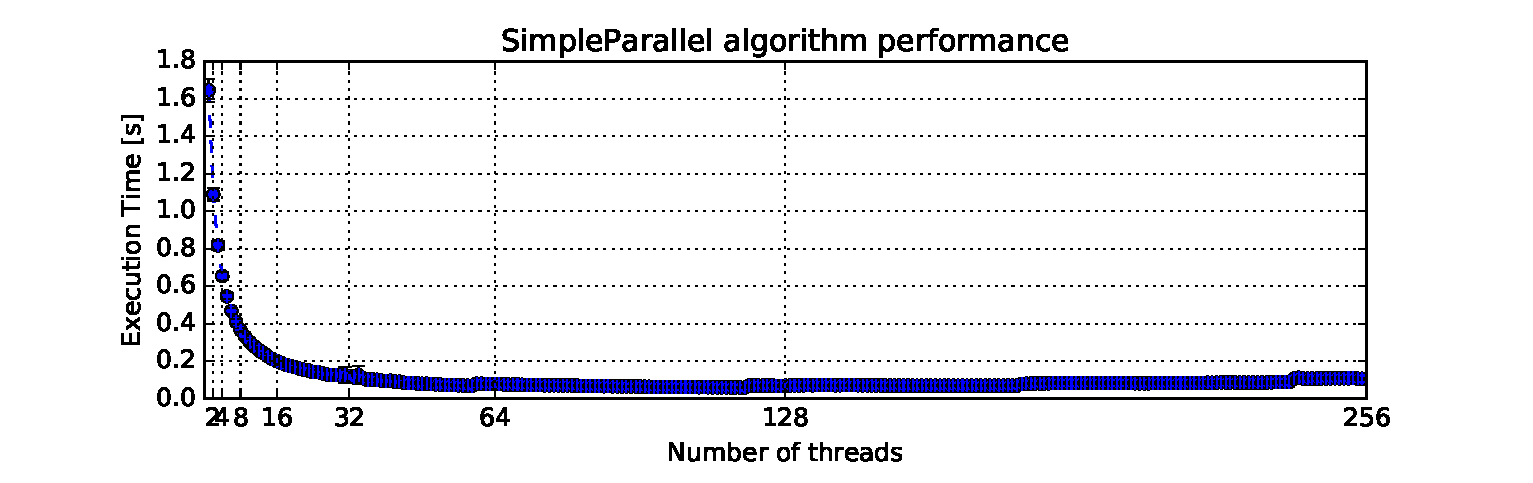
\includegraphics[scale=0.33]{./plots/total.eps}
  \caption{Execution time of Simple algorithm for a square of 10$^7$ points\label{SimpleParallel Total}}
\end{figure}



\section{Conclusions}

We implemented three parallel algorithms for solving the convex hull problem and as a general remark we believe that all the considered algorithms are valid and allow good performance under different conditions (input size, shape and number of processing threads).
One of the algorithms (\textit{HullTree}), however, doesn't work nicely with very large resulting hulls (like with circles as input sets).

We were able to obtain superlinear speedup using randomly generated points in a squared interval %TODO more accurate world%
and close to linear with two of the three algorithms using a circle as input.

Generally speaking, we could say the parallelization of the convex hull problem allows significant improvements in performance with bigger input sets and with a not-too-large number of processing threads.

Even though we oly considered square, disk and circle as shapes for the input set, these algorithms can be used for any ordered input set with distinct $x$ coordinate and their performance should be similar to the one we had with the analyzed shapes (i.e. similar to circle's one if most of the points in the input set takes part to the final hull, else similar to disk and square's ones).

\section{Further comments}

Here we provide some further tips.

\mypar{Further general guidelines}

\begin{itemize}
\item For short papers, to save space, I use paragraph titles instead of
subsections, as shown in the introduction.

\item It is generally a good idea to break sections into such smaller
units for readability and since it helps you to (visually) structure the story.

\item The above section titles should be adapted to more precisely
reflect what you do.

\item Each section should be started with a very
short summary of what the reader can expect in this section. Nothing
more awkward as when the story starts and one does not know what the
direction is or the goal.

\item Make sure you define every acronym you use, no matter how
convinced you are the reader knows it.

\item Always spell-check before you submit (to us in this case).

\item Be picky. When writing a paper you should always strive for very
high quality. Many people may read it and the quality makes a big difference.
In this class, the quality is part of the grade.

\item Books helping you to write better: \cite{Higham:98} and \cite{Strunk:00}.

\item Conversion to pdf (latex users only): 

dvips -o conference.ps -t letter -Ppdf -G0 conference.dvi

and then

ps2pdf conference.ps
\end{itemize}

\mypar{Graphics} For plots that are not images {\em never} generate the bitmap formats
jpeg, gif, bmp, tif. Use eps, which means encapsulate postscript. It is
scalable since it is a vector graphic description of your graph. E.g.,
from Matlab, you can export to eps.

The format pdf is also fine for plots (you need pdflatex then), but only if the plot was never before in the format 
jpeg, gif, bmp, tif.


% References should be produced using the bibtex program from suitable
% BiBTeX files (here: bibl_conf). The IEEEbib.bst bibliography
% style file from IEEE produces unsorted bibliography list.
% -------------------------------------------------------------------------
\bibliographystyle{IEEEbib}
\bibliography{bibl_conf}

\end{document}

